% This file was adapted from ICLR2022_conference.tex example provided for the ICLR conference
\documentclass{article} % For LaTeX2e
\usepackage{collas2025_conference,times}
\usepackage{easyReview}

% Optional math commands from https://github.com/goodfeli/dlbook_notation.
%%%%% NEW MATH DEFINITIONS %%%%%

\usepackage{amsmath,amsfonts,bm}

% Mark sections of captions for referring to divisions of figures
\newcommand{\figleft}{{\em (Left)}}
\newcommand{\figcenter}{{\em (Center)}}
\newcommand{\figright}{{\em (Right)}}
\newcommand{\figtop}{{\em (Top)}}
\newcommand{\figbottom}{{\em (Bottom)}}
\newcommand{\captiona}{{\em (a)}}
\newcommand{\captionb}{{\em (b)}}
\newcommand{\captionc}{{\em (c)}}
\newcommand{\captiond}{{\em (d)}}

% Highlight a newly defined term
\newcommand{\newterm}[1]{{\bf #1}}


% Figure reference, lower-case.
\def\figref#1{figure~\ref{#1}}
% Figure reference, capital. For start of sentence
\def\Figref#1{Figure~\ref{#1}}
\def\twofigref#1#2{figures \ref{#1} and \ref{#2}}
\def\quadfigref#1#2#3#4{figures \ref{#1}, \ref{#2}, \ref{#3} and \ref{#4}}
% Section reference, lower-case.
\def\secref#1{section~\ref{#1}}
% Section reference, capital.
\def\Secref#1{Section~\ref{#1}}
% Reference to two sections.
\def\twosecrefs#1#2{sections \ref{#1} and \ref{#2}}
% Reference to three sections.
\def\secrefs#1#2#3{sections \ref{#1}, \ref{#2} and \ref{#3}}
% Reference to an equation, lower-case.
\def\eqref#1{equation~\ref{#1}}
% Reference to an equation, upper case
\def\Eqref#1{Equation~\ref{#1}}
% A raw reference to an equation---avoid using if possible
\def\plaineqref#1{\ref{#1}}
% Reference to a chapter, lower-case.
\def\chapref#1{chapter~\ref{#1}}
% Reference to an equation, upper case.
\def\Chapref#1{Chapter~\ref{#1}}
% Reference to a range of chapters
\def\rangechapref#1#2{chapters\ref{#1}--\ref{#2}}
% Reference to an algorithm, lower-case.
\def\algref#1{algorithm~\ref{#1}}
% Reference to an algorithm, upper case.
\def\Algref#1{Algorithm~\ref{#1}}
\def\twoalgref#1#2{algorithms \ref{#1} and \ref{#2}}
\def\Twoalgref#1#2{Algorithms \ref{#1} and \ref{#2}}
% Reference to a part, lower case
\def\partref#1{part~\ref{#1}}
% Reference to a part, upper case
\def\Partref#1{Part~\ref{#1}}
\def\twopartref#1#2{parts \ref{#1} and \ref{#2}}

\def\ceil#1{\lceil #1 \rceil}
\def\floor#1{\lfloor #1 \rfloor}
\def\1{\bm{1}}
\newcommand{\train}{\mathcal{D}}
\newcommand{\valid}{\mathcal{D_{\mathrm{valid}}}}
\newcommand{\test}{\mathcal{D_{\mathrm{test}}}}

\def\eps{{\epsilon}}


% Random variables
\def\reta{{\textnormal{$\eta$}}}
\def\ra{{\textnormal{a}}}
\def\rb{{\textnormal{b}}}
\def\rc{{\textnormal{c}}}
\def\rd{{\textnormal{d}}}
\def\re{{\textnormal{e}}}
\def\rf{{\textnormal{f}}}
\def\rg{{\textnormal{g}}}
\def\rh{{\textnormal{h}}}
\def\ri{{\textnormal{i}}}
\def\rj{{\textnormal{j}}}
\def\rk{{\textnormal{k}}}
\def\rl{{\textnormal{l}}}
% rm is already a command, just don't name any random variables m
\def\rn{{\textnormal{n}}}
\def\ro{{\textnormal{o}}}
\def\rp{{\textnormal{p}}}
\def\rq{{\textnormal{q}}}
\def\rr{{\textnormal{r}}}
\def\rs{{\textnormal{s}}}
\def\rt{{\textnormal{t}}}
\def\ru{{\textnormal{u}}}
\def\rv{{\textnormal{v}}}
\def\rw{{\textnormal{w}}}
\def\rx{{\textnormal{x}}}
\def\ry{{\textnormal{y}}}
\def\rz{{\textnormal{z}}}

% Random vectors
\def\rvepsilon{{\mathbf{\epsilon}}}
\def\rvtheta{{\mathbf{\theta}}}
\def\rva{{\mathbf{a}}}
\def\rvb{{\mathbf{b}}}
\def\rvc{{\mathbf{c}}}
\def\rvd{{\mathbf{d}}}
\def\rve{{\mathbf{e}}}
\def\rvf{{\mathbf{f}}}
\def\rvg{{\mathbf{g}}}
\def\rvh{{\mathbf{h}}}
\def\rvu{{\mathbf{i}}}
\def\rvj{{\mathbf{j}}}
\def\rvk{{\mathbf{k}}}
\def\rvl{{\mathbf{l}}}
\def\rvm{{\mathbf{m}}}
\def\rvn{{\mathbf{n}}}
\def\rvo{{\mathbf{o}}}
\def\rvp{{\mathbf{p}}}
\def\rvq{{\mathbf{q}}}
\def\rvr{{\mathbf{r}}}
\def\rvs{{\mathbf{s}}}
\def\rvt{{\mathbf{t}}}
\def\rvu{{\mathbf{u}}}
\def\rvv{{\mathbf{v}}}
\def\rvw{{\mathbf{w}}}
\def\rvx{{\mathbf{x}}}
\def\rvy{{\mathbf{y}}}
\def\rvz{{\mathbf{z}}}

% Elements of random vectors
\def\erva{{\textnormal{a}}}
\def\ervb{{\textnormal{b}}}
\def\ervc{{\textnormal{c}}}
\def\ervd{{\textnormal{d}}}
\def\erve{{\textnormal{e}}}
\def\ervf{{\textnormal{f}}}
\def\ervg{{\textnormal{g}}}
\def\ervh{{\textnormal{h}}}
\def\ervi{{\textnormal{i}}}
\def\ervj{{\textnormal{j}}}
\def\ervk{{\textnormal{k}}}
\def\ervl{{\textnormal{l}}}
\def\ervm{{\textnormal{m}}}
\def\ervn{{\textnormal{n}}}
\def\ervo{{\textnormal{o}}}
\def\ervp{{\textnormal{p}}}
\def\ervq{{\textnormal{q}}}
\def\ervr{{\textnormal{r}}}
\def\ervs{{\textnormal{s}}}
\def\ervt{{\textnormal{t}}}
\def\ervu{{\textnormal{u}}}
\def\ervv{{\textnormal{v}}}
\def\ervw{{\textnormal{w}}}
\def\ervx{{\textnormal{x}}}
\def\ervy{{\textnormal{y}}}
\def\ervz{{\textnormal{z}}}

% Random matrices
\def\rmA{{\mathbf{A}}}
\def\rmB{{\mathbf{B}}}
\def\rmC{{\mathbf{C}}}
\def\rmD{{\mathbf{D}}}
\def\rmE{{\mathbf{E}}}
\def\rmF{{\mathbf{F}}}
\def\rmG{{\mathbf{G}}}
\def\rmH{{\mathbf{H}}}
\def\rmI{{\mathbf{I}}}
\def\rmJ{{\mathbf{J}}}
\def\rmK{{\mathbf{K}}}
\def\rmL{{\mathbf{L}}}
\def\rmM{{\mathbf{M}}}
\def\rmN{{\mathbf{N}}}
\def\rmO{{\mathbf{O}}}
\def\rmP{{\mathbf{P}}}
\def\rmQ{{\mathbf{Q}}}
\def\rmR{{\mathbf{R}}}
\def\rmS{{\mathbf{S}}}
\def\rmT{{\mathbf{T}}}
\def\rmU{{\mathbf{U}}}
\def\rmV{{\mathbf{V}}}
\def\rmW{{\mathbf{W}}}
\def\rmX{{\mathbf{X}}}
\def\rmY{{\mathbf{Y}}}
\def\rmZ{{\mathbf{Z}}}

% Elements of random matrices
\def\ermA{{\textnormal{A}}}
\def\ermB{{\textnormal{B}}}
\def\ermC{{\textnormal{C}}}
\def\ermD{{\textnormal{D}}}
\def\ermE{{\textnormal{E}}}
\def\ermF{{\textnormal{F}}}
\def\ermG{{\textnormal{G}}}
\def\ermH{{\textnormal{H}}}
\def\ermI{{\textnormal{I}}}
\def\ermJ{{\textnormal{J}}}
\def\ermK{{\textnormal{K}}}
\def\ermL{{\textnormal{L}}}
\def\ermM{{\textnormal{M}}}
\def\ermN{{\textnormal{N}}}
\def\ermO{{\textnormal{O}}}
\def\ermP{{\textnormal{P}}}
\def\ermQ{{\textnormal{Q}}}
\def\ermR{{\textnormal{R}}}
\def\ermS{{\textnormal{S}}}
\def\ermT{{\textnormal{T}}}
\def\ermU{{\textnormal{U}}}
\def\ermV{{\textnormal{V}}}
\def\ermW{{\textnormal{W}}}
\def\ermX{{\textnormal{X}}}
\def\ermY{{\textnormal{Y}}}
\def\ermZ{{\textnormal{Z}}}

% Vectors
\def\vzero{{\bm{0}}}
\def\vone{{\bm{1}}}
\def\vmu{{\bm{\mu}}}
\def\vtheta{{\bm{\theta}}}
\def\va{{\bm{a}}}
\def\vb{{\bm{b}}}
\def\vc{{\bm{c}}}
\def\vd{{\bm{d}}}
\def\ve{{\bm{e}}}
\def\vf{{\bm{f}}}
\def\vg{{\bm{g}}}
\def\vh{{\bm{h}}}
\def\vi{{\bm{i}}}
\def\vj{{\bm{j}}}
\def\vk{{\bm{k}}}
\def\vl{{\bm{l}}}
\def\vm{{\bm{m}}}
\def\vn{{\bm{n}}}
\def\vo{{\bm{o}}}
\def\vp{{\bm{p}}}
\def\vq{{\bm{q}}}
\def\vr{{\bm{r}}}
\def\vs{{\bm{s}}}
\def\vt{{\bm{t}}}
\def\vu{{\bm{u}}}
\def\vv{{\bm{v}}}
\def\vw{{\bm{w}}}
\def\vx{{\bm{x}}}
\def\vy{{\bm{y}}}
\def\vz{{\bm{z}}}

% Elements of vectors
\def\evalpha{{\alpha}}
\def\evbeta{{\beta}}
\def\evepsilon{{\epsilon}}
\def\evlambda{{\lambda}}
\def\evomega{{\omega}}
\def\evmu{{\mu}}
\def\evpsi{{\psi}}
\def\evsigma{{\sigma}}
\def\evtheta{{\theta}}
\def\eva{{a}}
\def\evb{{b}}
\def\evc{{c}}
\def\evd{{d}}
\def\eve{{e}}
\def\evf{{f}}
\def\evg{{g}}
\def\evh{{h}}
\def\evi{{i}}
\def\evj{{j}}
\def\evk{{k}}
\def\evl{{l}}
\def\evm{{m}}
\def\evn{{n}}
\def\evo{{o}}
\def\evp{{p}}
\def\evq{{q}}
\def\evr{{r}}
\def\evs{{s}}
\def\evt{{t}}
\def\evu{{u}}
\def\evv{{v}}
\def\evw{{w}}
\def\evx{{x}}
\def\evy{{y}}
\def\evz{{z}}

% Matrix
\def\mA{{\bm{A}}}
\def\mB{{\bm{B}}}
\def\mC{{\bm{C}}}
\def\mD{{\bm{D}}}
\def\mE{{\bm{E}}}
\def\mF{{\bm{F}}}
\def\mG{{\bm{G}}}
\def\mH{{\bm{H}}}
\def\mI{{\bm{I}}}
\def\mJ{{\bm{J}}}
\def\mK{{\bm{K}}}
\def\mL{{\bm{L}}}
\def\mM{{\bm{M}}}
\def\mN{{\bm{N}}}
\def\mO{{\bm{O}}}
\def\mP{{\bm{P}}}
\def\mQ{{\bm{Q}}}
\def\mR{{\bm{R}}}
\def\mS{{\bm{S}}}
\def\mT{{\bm{T}}}
\def\mU{{\bm{U}}}
\def\mV{{\bm{V}}}
\def\mW{{\bm{W}}}
\def\mX{{\bm{X}}}
\def\mY{{\bm{Y}}}
\def\mZ{{\bm{Z}}}
\def\mBeta{{\bm{\beta}}}
\def\mPhi{{\bm{\Phi}}}
\def\mLambda{{\bm{\Lambda}}}
\def\mSigma{{\bm{\Sigma}}}

% Tensor
\DeclareMathAlphabet{\mathsfit}{\encodingdefault}{\sfdefault}{m}{sl}
\SetMathAlphabet{\mathsfit}{bold}{\encodingdefault}{\sfdefault}{bx}{n}
\newcommand{\tens}[1]{\bm{\mathsfit{#1}}}
\def\tA{{\tens{A}}}
\def\tB{{\tens{B}}}
\def\tC{{\tens{C}}}
\def\tD{{\tens{D}}}
\def\tE{{\tens{E}}}
\def\tF{{\tens{F}}}
\def\tG{{\tens{G}}}
\def\tH{{\tens{H}}}
\def\tI{{\tens{I}}}
\def\tJ{{\tens{J}}}
\def\tK{{\tens{K}}}
\def\tL{{\tens{L}}}
\def\tM{{\tens{M}}}
\def\tN{{\tens{N}}}
\def\tO{{\tens{O}}}
\def\tP{{\tens{P}}}
\def\tQ{{\tens{Q}}}
\def\tR{{\tens{R}}}
\def\tS{{\tens{S}}}
\def\tT{{\tens{T}}}
\def\tU{{\tens{U}}}
\def\tV{{\tens{V}}}
\def\tW{{\tens{W}}}
\def\tX{{\tens{X}}}
\def\tY{{\tens{Y}}}
\def\tZ{{\tens{Z}}}


% Graph
\def\gA{{\mathcal{A}}}
\def\gB{{\mathcal{B}}}
\def\gC{{\mathcal{C}}}
\def\gD{{\mathcal{D}}}
\def\gE{{\mathcal{E}}}
\def\gF{{\mathcal{F}}}
\def\gG{{\mathcal{G}}}
\def\gH{{\mathcal{H}}}
\def\gI{{\mathcal{I}}}
\def\gJ{{\mathcal{J}}}
\def\gK{{\mathcal{K}}}
\def\gL{{\mathcal{L}}}
\def\gM{{\mathcal{M}}}
\def\gN{{\mathcal{N}}}
\def\gO{{\mathcal{O}}}
\def\gP{{\mathcal{P}}}
\def\gQ{{\mathcal{Q}}}
\def\gR{{\mathcal{R}}}
\def\gS{{\mathcal{S}}}
\def\gT{{\mathcal{T}}}
\def\gU{{\mathcal{U}}}
\def\gV{{\mathcal{V}}}
\def\gW{{\mathcal{W}}}
\def\gX{{\mathcal{X}}}
\def\gY{{\mathcal{Y}}}
\def\gZ{{\mathcal{Z}}}

% Sets
\def\sA{{\mathbb{A}}}
\def\sB{{\mathbb{B}}}
\def\sC{{\mathbb{C}}}
\def\sD{{\mathbb{D}}}
% Don't use a set called E, because this would be the same as our symbol
% for expectation.
\def\sF{{\mathbb{F}}}
\def\sG{{\mathbb{G}}}
\def\sH{{\mathbb{H}}}
\def\sI{{\mathbb{I}}}
\def\sJ{{\mathbb{J}}}
\def\sK{{\mathbb{K}}}
\def\sL{{\mathbb{L}}}
\def\sM{{\mathbb{M}}}
\def\sN{{\mathbb{N}}}
\def\sO{{\mathbb{O}}}
\def\sP{{\mathbb{P}}}
\def\sQ{{\mathbb{Q}}}
\def\sR{{\mathbb{R}}}
\def\sS{{\mathbb{S}}}
\def\sT{{\mathbb{T}}}
\def\sU{{\mathbb{U}}}
\def\sV{{\mathbb{V}}}
\def\sW{{\mathbb{W}}}
\def\sX{{\mathbb{X}}}
\def\sY{{\mathbb{Y}}}
\def\sZ{{\mathbb{Z}}}

% Entries of a matrix
\def\emLambda{{\Lambda}}
\def\emA{{A}}
\def\emB{{B}}
\def\emC{{C}}
\def\emD{{D}}
\def\emE{{E}}
\def\emF{{F}}
\def\emG{{G}}
\def\emH{{H}}
\def\emI{{I}}
\def\emJ{{J}}
\def\emK{{K}}
\def\emL{{L}}
\def\emM{{M}}
\def\emN{{N}}
\def\emO{{O}}
\def\emP{{P}}
\def\emQ{{Q}}
\def\emR{{R}}
\def\emS{{S}}
\def\emT{{T}}
\def\emU{{U}}
\def\emV{{V}}
\def\emW{{W}}
\def\emX{{X}}
\def\emY{{Y}}
\def\emZ{{Z}}
\def\emSigma{{\Sigma}}

% entries of a tensor
% Same font as tensor, without \bm wrapper
\newcommand{\etens}[1]{\mathsfit{#1}}
\def\etLambda{{\etens{\Lambda}}}
\def\etA{{\etens{A}}}
\def\etB{{\etens{B}}}
\def\etC{{\etens{C}}}
\def\etD{{\etens{D}}}
\def\etE{{\etens{E}}}
\def\etF{{\etens{F}}}
\def\etG{{\etens{G}}}
\def\etH{{\etens{H}}}
\def\etI{{\etens{I}}}
\def\etJ{{\etens{J}}}
\def\etK{{\etens{K}}}
\def\etL{{\etens{L}}}
\def\etM{{\etens{M}}}
\def\etN{{\etens{N}}}
\def\etO{{\etens{O}}}
\def\etP{{\etens{P}}}
\def\etQ{{\etens{Q}}}
\def\etR{{\etens{R}}}
\def\etS{{\etens{S}}}
\def\etT{{\etens{T}}}
\def\etU{{\etens{U}}}
\def\etV{{\etens{V}}}
\def\etW{{\etens{W}}}
\def\etX{{\etens{X}}}
\def\etY{{\etens{Y}}}
\def\etZ{{\etens{Z}}}

% The true underlying data generating distribution
\newcommand{\pdata}{p_{\rm{data}}}
% The empirical distribution defined by the training set
\newcommand{\ptrain}{\hat{p}_{\rm{data}}}
\newcommand{\Ptrain}{\hat{P}_{\rm{data}}}
% The model distribution
\newcommand{\pmodel}{p_{\rm{model}}}
\newcommand{\Pmodel}{P_{\rm{model}}}
\newcommand{\ptildemodel}{\tilde{p}_{\rm{model}}}
% Stochastic autoencoder distributions
\newcommand{\pencode}{p_{\rm{encoder}}}
\newcommand{\pdecode}{p_{\rm{decoder}}}
\newcommand{\precons}{p_{\rm{reconstruct}}}

\newcommand{\laplace}{\mathrm{Laplace}} % Laplace distribution

\newcommand{\E}{\mathbb{E}}
\newcommand{\Ls}{\mathcal{L}}
\newcommand{\R}{\mathbb{R}}
\newcommand{\emp}{\tilde{p}}
\newcommand{\lr}{\alpha}
\newcommand{\reg}{\lambda}
\newcommand{\rect}{\mathrm{rectifier}}
\newcommand{\softmax}{\mathrm{softmax}}
\newcommand{\sigmoid}{\sigma}
\newcommand{\softplus}{\zeta}
\newcommand{\KL}{D_{\mathrm{KL}}}
\newcommand{\Var}{\mathrm{Var}}
\newcommand{\standarderror}{\mathrm{SE}}
\newcommand{\Cov}{\mathrm{Cov}}
% Wolfram Mathworld says $L^2$ is for function spaces and $\ell^2$ is for vectors
% But then they seem to use $L^2$ for vectors throughout the site, and so does
% wikipedia.
\newcommand{\normlzero}{L^0}
\newcommand{\normlone}{L^1}
\newcommand{\normltwo}{L^2}
\newcommand{\normlp}{L^p}
\newcommand{\normmax}{L^\infty}

\newcommand{\parents}{Pa} % See usage in notation.tex. Chosen to match Daphne's book.

\DeclareMathOperator*{\argmax}{arg\,max}
\DeclareMathOperator*{\argmin}{arg\,min}

\DeclareMathOperator{\sign}{sign}
\DeclareMathOperator{\Tr}{Tr}
\let\ab\allowbreak


% Please leave these options as they are
\usepackage{hyperref}
\hypersetup{
    colorlinks=true,
    linkcolor=red,
    filecolor=magenta,
    urlcolor=blue,
    citecolor=purple,
    pdftitle={Overleaf Example},
    pdfpagemode=FullScreen,
    }




\title{Ephemeral Memory: \\ Successful retention of short-term information using variable plasticity and decaying weight values}

% Authors must not appear in the submitted version. They should be hidden
% as long as the \collasfinalcopy macro remains commented out below.
% Non-anonymous submissions will be rejected without review.

\author{
  Jaden Lorenc \\
  Computer Science Department \\
  Brigham Young University \\
  \texttt{jaden.lorenc@byu.edu}
}


% The \author macro works with any number of authors. There are two commands
% used to separate the names and addresses of multiple authors: \And and \AND.
%
% Using \And between authors leaves it to \LaTeX{} to determine where to break
% the lines. Using \AND forces a linebreak at that point. So, if \LaTeX{}
% puts 3 of 4 authors names on the first line, and the last on the second
% line, try using \AND instead of \And before the third author name.

\newcommand{\fix}{\marginpar{FIX}}
\newcommand{\new}{\marginpar{NEW}}

%\collasfinalcopy % Uncomment for camera-ready version, but NOT for submission.

%\preprintcopy % Uncomment for the preprint version, but NOT for submission.

\begin{document}


\maketitle

% \documentclass{article}
% \usepackage{collas2025_conference}
% \usepackage{times}
% \usepackage{amsmath}
% \usepackage{amssymb}
% \usepackage{graphicx}
% \usepackage{hyperref}

% \title{Ephemeral Weights: Storing Short-Term Memory in Neural Network Parameters}

% \author{
%   \textbf{Author Names}\\
%   Institution\\
%   \texttt{email@example.com}
% }

% \begin{document}

\maketitle

\begin{abstract}
A few weights with quickly decaying values and high learning rates can replace the hidden, recurrent connection in an RNN, storing short-term memory in the parameters themselves via a standard loss calculation and backpropagation gradient calculation. In most artificial neural network (ANN) designs, the gradient update mechanism (loss function and backpropagation) is viewed as a process distinct from the forward pass, with one generating predictions and the other computing and applying parameter updates. However, error computation and backpropagation can be repurposed for use as short-term memory. This is done by designating a fraction of the model’s weights as “fast weights,” endowed with larger learning rates to enable swift adaptation and decay to prevent gradient instability. The result is a constantly updating record of recent gradient updates directly accessible to the network’s weights, negating the need for rolling context windows or recurrent connections. This approach enables short-term context to be stored purely in ephemeral, rapidly updated parameters, offering a more direct route from manually stored memory to parameter-based memory. We demonstrate this approach on character-level sequence prediction tasks, showing that our ephemeral weights model can successfully solve key-recall, repeated sequence, and reversed sequence tasks without any recurrent connections, achieving comparable accuracy to traditional RNNs. The approach establishes that continuous state information can be propagated solely through parameter updates; hence the use of static plasticity and the removal of recurrent connections, allowing the existing weight update mechanism to encode both long and short-term information.
\end{abstract}

\section{Introduction}

While it is typical to consider the loss function and backpropagation as distinct from the forward pass components of an artificial neural net (ANN), it may be constructive to consider their permanent inclusion in the structure of the model, to be used even at inference-time. Error computation and backpropagation can be repurposed for use as a form of short-term memory, even to the point of replacing the hidden connection in a recurrent neural network (RNN). To do so necessitates varying degrees of plasticity among the parameters of the neural network, so that both long-term gradient descent can continue to improve the overall performance of the model, while faster-changing parameters grant the ability to encode short-term information. A simple way to do this is by designating a fraction of the parameters Ephemeral Weights, and giving them a larger learning rate. They also need a rate of decay in order to prevent gradient instability and eventual explosion. The result is a constantly updating record of recent gradient updates received from the loss function, directly accessible to the weights of the model. This parameter based record can replace the recurrent connection in a Recurrent Neural Network (RNN), allowing the existing weight update mechanism to encode \emph{both} long and short-term information.

The purpose of this paper is to establish that simple ephemeral weights are able to replace a recurrent connection in sequence prediction tasks. They store short-term context in the parameters themselves of a neural network, using existing weight update algorithms. The loss function, backpropagation of errors, and gradient descent are repurposed for rapid online learning of the current task and its relevant data. The paradigm renders those weight update mechanisms inseparable from the model, even at inference time. Future neural networks likely will use a more sophisticated weight plasticity scheme, alongside the recurrent connections and context windows used in modern setups. Ephemeral weights show that there may exist a more gradual transition from the more manually stored memory to parameter-based memory.

The contributions of this paper are as follows: 
(1) We introduce ephemeral weights, a novel approach that repurposes standard backpropagation to store short-term context directly within a neural network's parameters, 
(2) We demonstrate that designating a small fraction of network parameters as ``ephemeral weights'', a variant of fast weights, with higher learning rates can enable memory functions without recurrent connections, 
(3) We identify the gradient norm ratio between high and low-plasticity weights as a key early warning indicator for system instability, providing mechanistic insight into the volatility dynamics, 
(4) We show that dual-timescale learning can be achieved where low-plasticity weights maintain stable long-term learning while high-plasticity weights manage volatile working memory without mutual interference, 
(5) We provide comprehensive analysis of implementation requirements including gradient propagation methods, batching constraints, and stabilization strategies essential for practical deployment, 
(6) We empirically demonstrate success on key-recall, repeated sequence, and reversed sequence working memory tasks, achieving comparable accuracy to traditional RNNs, with parametric memory replacing the recurrent connections.

\section{Related Works}

\subsection{Contextual, Online, and Meta-Learning}

A variety of approaches modify neural networks to maintain information beyond their immediate inputs, either by changing parameters during inference or adding explicit memory structures. While these methods don't necessarily focus on encoding short-term memories in parameters themselves, they meet related challenges.

\subsubsection{Parameter-Based Adaptation}

Meta-learning research focuses on creating models that can quickly adapt themselves to novel circumstances. These approaches typically involve an inner and outer training loop structure. As \citet{finnModelagnosticMetalearningFast2017} demonstrated with MAML, the outer loop optimizes for initial parameters that can rapidly adapt to new tasks in the inner loop. However, the computational challenges are significant—the outer training loop is often not well-suited for backpropagation-based gradient calculations since it would require storing activations for an infeasible number of parameters. Thus, evolutionary learning or other alternatives are commonly used, with traditional backpropagation typically limited to very small inner loop models.

In continual and online learning, models must adapt to new data without forgetting previous knowledge—a capability that standard neural networks struggle with due to the rigid training/inference paradigm. A common approach is experience replay, where past experiences are stored and periodically revisited. Popularized in deep Q-networks by \citet{mnihHumanlevelControlDeep2015}, replay buffers stabilize training and improve data efficiency by breaking temporal correlations in online data. However, this solution adds complexity through buffer management and sampling strategies.

As recent works confirm \citet{Forgetting_Survey_2024}, memory-based rehearsal provides a strong baseline in lifelong learning but requires extra storage and training iterations that simpler online learners would avoid. More sophisticated replay variants (selective storing, compressed activation replay, or generative replay) further increase system complexity by introducing components solely to manage past knowledge. This represents a fundamental trade-off: simplicity versus the ability to retain information across learning episodes.

\subsubsection{External Memory Architectures}

Rather than modifying learning algorithms, some approaches augment neural networks with explicit memory structures. Neural Turing Machines (NTM), introduced by \citet{Graves2014NeuralTM}, pair a neural controller with a read-write memory matrix, allowing networks to store and retrieve information over extended sequences. This design enables algorithmic tasks like copying or sorting that standard RNNs cannot perform. However, the controller must learn where to write or read, making training more resource-intensive and complex. While subsequent variants like the Differentiable Neural Computer refined these mechanisms, they still struggled with consistency and scalability over very long sequences.

Building on these foundations, \citet{westonMemoryNetworks2014} introduced Memory Networks for question-answering tasks, using a separate memory to store facts with an iterative attention process for retrieval. Similarly, \citet{santoroMetaLearningMemoryAugmentedNeural2016} showed that Memory-Augmented Neural Networks (MANN) can rapidly encode new samples into external memory, achieving one-shot learning without extensive retraining. The trade-off is an extra memory module and controller logic that simpler feed-forward networks don't require.

In recent years, transformer-based models have also incorporated external memory systems. \citet{wuMemorizingTransformers2022} proposed Memorizing Transformers that maintain a key-value store of past activations, extending the effective context window beyond fixed self-attention limits. Similarly, \citet{wangAugmentingLanguageModels2023} augmented language models with dedicated long-term memory modules that require learning separate read/write operations. These approaches improve knowledge retention but add complexity through additional networks and procedures.

\subsubsection{Current Industry Approaches and Limitations}

The mainstream AI industry often approaches these challenges backward, with a renewed focus on inference-time compute that optimizes for the exclusion of training loop components. Fine-tuning serves as a workaround for the constraints of static, non-learning models. Parameter-efficient fine-tuning techniques allow for more space-efficient incorporation of new knowledge, while retrieval-augmented generation (RAG) addresses limitations in context window capacity by retrieving external information. Attention mechanisms on limited-length context windows solve short-term memory challenges by simply preserving all information and performing expensive relevance computations.

Recent state-space models like Mamba and Hyena attempt to address these limitations but create lossy representations of context. RWKV aims to apply attention-like mechanisms to true RNNs but still faces long-term dependency challenges similar to LSTM, GRU, and vanilla RNN architectures—causing generated outputs to easily veer from context.

We can view the attention mechanism itself as a form of meta-learning that dynamically generates weights for a linear layer. In contrast, our approach with ephemeral weights generates only changes to a limited number of highly flexible parameters, potentially offering a more direct and efficient route to parameter-based short-term memory without the architectural complexity of dedicated memory modules or the algorithmic overhead of experience replay.

\subsection{Dynamic Parameter Adaptation and Fast Weights}

The concept of rapidly updated parameters in neural networks has been explored through various complementary approaches. These techniques enable online adaptation by making parameters dynamic, effectively treating short-term weight changes as a form of memory. While traditional neural networks maintain static weights after training, techniques like fast weights, hypernetworks, and differentiable plasticity allow certain parameters to update rapidly in response to new inputs or tasks, adding a form of in-network memory stored in temporary weight changes.

Fast weights have a long history in neural network research, dating back to \citet{hintonUsingFastWeights1987}, who described a dual weight architecture where each weight is mirrored by one with a higher learning rate that decays toward zero. The `effective' weight for each forward pass is the sum of these fast and slow weights, with the original goal being to \emph{deblur} old associations rather than explicitly encode short-term information. \citet{schmidhuberLearningControlFastweight1992} further developed this concept, drawing inspiration from biological short-term synaptic plasticity to create secondary weights that update based on recent activity.

Modern implementations of this idea take various forms. \citet{miconiDifferentiablePlasticityTraining2018a} implemented differentiable Hebbian plasticity, where each synapse has a plastic component adjusted with a Hebb rule during forward passes, with the \emph{degree} of plasticity learned through gradient descent. This enables the network to memorize recent patterns by temporarily modifying weights, allowing it to succeed at tasks like one-shot recall that static networks fail at. Their plastic recurrent networks demonstrated the ability to memorize high-dimensional images seen during testing, whereas non-plastic counterparts couldn't—highlighting the benefit of this added complexity.

Hypernetworks extend this idea by using one neural network to generate the weights of another. Fast Weight Programmers (FWP) apply this concept to compute weight changes at each step, with a meta network continually emitting rapid parameter updates for the main network. As  \citet{irieGoingLinearTransformers2021a} demonstrated, these rapid updates can serve as an alternative to recurrent connections, with current enhancements making FWPs competitive with modern architectures. \citet{baUsingFastWeights2016} took a different approach, generating fast weights based on both a hidden recurrent connection and decaying previous fast weights, replacing the hidden vector with one calculated through an iterative inner loop using a fast memory weight matrix.

While promising, hypernetworks introduce efficiency and learning challenges through their outer/inner loop structure. Each training iteration may require maintaining two sets of weights—the hypernetwork's and the generated network's—along with their respective gradients, significantly increasing memory usage and computational cost. The need to backpropagate through both loops can limit scalability, often necessitating specialized optimization strategies or approximations.

Another approach is dynamic evaluation, introduced by \citet{mikolovRecurrentNeuralNetwork2010} and refined by \citet{pmlr-v80-krause18a} for language models. Here, the model performs extra gradient updates on recent data during inference to improve next-word predictions. This yields lower perplexity on sequences by continuously adapting model parameters to recent tokens, at the cost of 3× or more computational overhead during inference. Dynamic evaluation makes inference much more complex (almost like a mini-training) compared to static models, since each step requires on-the-fly backpropagation.

\citet{finnModelagnosticMetalearningFast2017} formalized a meta-learning approach (MAML) to train models that can be quickly fine-tuned with a few gradient steps on a new task. While MAML doesn't add new network modules, it alters the training procedure to initialize the model in a state amenable to rapid parameter changes. This yields a form of short-term memory (the quick weight update) for new task information, though it requires second-order optimization during training and careful hyperparameter tuning.

A more recent innovation is Fast Weight Layers (FWL) by \citet{clark-etal-2022-meta}, which added to Transformers to emulate dynamic evaluation via learned linearized gradient updates. The FWL component learns to take the model's recent activations and "update" a set of fast weights through an attention mechanism that mirrors gradient descent, effectively giving the model a built-in one-step adaptation mechanism. This improves performance on language modeling, especially for rare or repeating tokens, but introduces an additional neural module atop the base model and a two-pass processing of each input.

Interestingly, multi-head attention can itself be viewed as a special case of fast weight programming. In attention, the ``fast weights// are effectively the key-value associations—an ephemeral weight matrix computed on the fly for each sequence of queries, then used immediately to transform them. This mirrors the fast-weight concept: a separate mechanism rapidly produces a parameter-like matrix to be used in the next computation step.

Overall, dynamic parameter strategies provide short-term memory by adjusting weights in response to new data, blurring the line between learning and inference. The recurring theme is that they outperform static models on adaptation-heavy tasks, but at the cost of more elaborate model architectures or training routines (e.g., meta-learning loops, auxiliary update networks) to manage these on-the-fly changes. The approach explored in this paper builds on these foundations, focusing on a minimal implementation of ephemeral weights that repurposes existing gradient calculation mechanisms for short-term memory storage.

\section{Methods}

\subsection{Biological Inspiration}

Our approach draws inspiration from biological mechanisms of synaptic plasticity, particularly Long-Term Potentiation (LTP). In biological neural networks, LTP induces a temporary strengthening of synapses that lasts approximately 1-6 hours, operating on a timescale between immediate neural firing and permanent structural changes. This process is mediated by calcium ion buildup, which both modulates the degree of plasticity and increases the likelihood of LTP occurring. This biological system provides a middle ground between immediate neural activation and permanent structural changes, allowing for information to be stored temporarily in the connection strengths themselves.

The ephemeral weights approach mimics this biological process by implementing parameters that rapidly adjust to recent inputs but gradually return to baseline—similar to how enhanced synaptic efficacy from LTP decays over hours if not reinforced. Just as the brain employs multiple timescales of memory storage (from millisecond neural firing to hours-long LTP to permanent structural changes), our model incorporates both fast-changing and stable parameters to create a more biologically plausible memory system.

\subsection{Model Architecture and Implementation}

Our experimental setup compares a traditional RNN with a novel model using ephemeral weights to store short-term memory. Both networks are character-level predictors trained on synthetic datasets designed to test memory capabilities.

\subsubsection{Baseline RNN Model}

The baseline is a standard RNN with a 3-layer architecture:

\begin{align}
h_t &= \text{ReLU}(W_{xh}x_t + W_{hh}h_{t-1} + b_h)\\
y_t &= \text{softmax}(W_{hy}h_t + b_y)
\end{align}

Where $h_t$ represents the hidden state at time $t$, $x_t$ is the one-hot encoded input character, $y_t$ is the output prediction, and $W_{xh}$, $W_{hh}$, $W_{hy}$ are weight matrices for input-to-hidden, hidden-to-hidden (recurrent), and hidden-to-output connections respectively. Each hidden layer contains 256 units.

\subsubsection{Ephemeral Weights Model}

Our proposed model eliminates the recurrent connection ($W_{hh}h_{t-1}$) entirely, replacing it with a mechanism for storing information in rapidly updating parameters. The architecture is:

\begin{align}
h_t &= \text{ReLU}(W_{xh}x_t + b_h)\\
y_t &= \text{softmax}(W_{hy}h_t + b_y)
\end{align}

Unlike traditional neural networks where parameters are fixed during inference, our model continues to update parameters even during evaluation, creating a parameter-based memory system.

\subsection{Ephemeral Weights Mechanism}

The core innovation is introducing variable learning rates across the network's parameters. Each weight $w_k$ is paired with a plasticity parameter $\alpha_k$ determining how quickly it responds to gradient signals. Parameters are divided into two categories:

\begin{enumerate}
\item \textbf{Slow weights} ($\alpha_k = 1$): Standard parameters that learn long-term patterns
\item \textbf{Ephemeral weights} ($\alpha_k = 10^4$ or $10^5$): Highly plastic parameters that rapidly encode recent information
\end{enumerate}

\begin{figure}[h]
\begin{center}
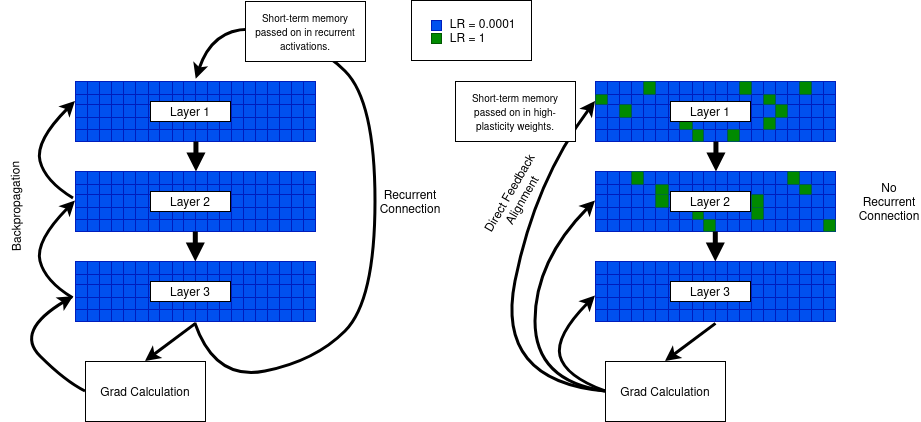
\includegraphics[width=0.8\linewidth]{model_diagram.png}
\caption{In a traditional RNN, the hidden state $h_{t-1}$ carries information forward through time. In the Ephemeral Weights model, this recurrent connection is removed, and short-term memory is instead stored in rapidly updating parameters (ephemeral weights) that adjust based on recent inputs. This allows the model to retain context without explicit recurrence.}
\label{fig:model_diagram}
\end{center}
\end{figure}

We randomly designate approximately 10\% of the total parameters as ephemeral weights, excluding the final output layer. The weight update rule follows:

\begin{equation}
w_k(t+1) = w_k(t) - \alpha_k \cdot \nabla_k L(t)
\end{equation}

Where $\nabla_k L(t)$ is the gradient of the loss function with respect to weight $w_k$ at time step $t$.

\subsection{Forgetting Rate Mechanism}

To prevent gradient instability from the rapid weight changes, we implement a controlled decay of ephemeral weights:

\begin{equation}
w_k^{\text{fast}}(t+1) = \gamma \cdot w_k^{\text{fast}}(t+1)
\end{equation}

Where $\gamma = 0.7$ is the forgetting rate coefficient applied after each standard update. This mechanism ensures that information stored in ephemeral weights gradually fades, maintaining stability while allowing the network to adapt to new inputs.

\subsection{Training Procedure}

Networks are trained using cross-entropy loss, with targets being the next character in the sequence. Both models use simple stochastic gradient descent (SGD) without additional optimizers. The learning rate is typically set to $1 \times 10^{-4}$ for both models, though experiments with the baseline RNN also use $1 \times 10^{-3}$ in some cases as noted in the Results section.

During both training and inference, the Ephemeral Weights model computes gradients and updates parameters after every character prediction, unlike traditional models where parameters remain fixed during inference. This continuous update cycle allows short-term contextual information to be encoded directly in the model parameters.

However, I will establish that continuous state information can be propagated solely through parameter updates; hence the use of static plasticity and the removal of recurrent connections.

\subsection{Implementation Details}

Several critical implementation considerations emerged during our experiments that significantly impact the stability and effectiveness of ephemeral weights.

\subsubsection{Gradient Propagation Methods}

Direct Feedback Alignment (DFA) demonstrates superior stability compared to standard backpropagation when used with ethereal weights. In DFA, feedback weights are randomly initialized for each layer and remain fixed throughout training, rather than using the network's own plastic weights for gradient propagation. This approach proves more stable because the fixed random weights avoid the volatility introduced when highly plastic parameters are used for both forward computation and backward gradient flow. Standard backpropagation with ethereal weights creates a volatile feedback loop where rapid weight changes amplify gradient instability.

\subsubsection{Character-Level Updates}

For short-term information to be effectively encoded, a complete training step—including loss calculation and backward pass—must be performed after each character prediction. This character-by-character update cycle is essential for the memory encoding mechanism, as it allows recent inputs to be immediately incorporated into the high-plasticity weights before the next prediction.

\subsubsection{Batching Constraints}

Traditional batching approaches fail with ethereal weights because they cause working memory to be shared across different sequence instances, obfuscating the information that should be encoded in high-plasticity weights. Instead, batching must be implemented using separate weight instances for each sequence, with gradient accumulation occurring only after complete sequences are processed. This ensures that each sequence maintains its own isolated working memory state.

\subsubsection{Stabilization Techniques}

Weight clipping emerges as an effective stabilization method, particularly for models using standard backpropagation. By constraining weight magnitudes, clipping helps control the volatile behavior that can arise from the aggressive gradient amplification inherent in the ethereal weights mechanism. However, gradient clipping proves ineffective, as the memory mechanism depends on occasional large gradient magnitudes to encode temporary information effectively.

Batch normalization and layer normalization are similarly counterproductive, as they normalize away the bimodal gradient distribution that is fundamental to the ethereal weights approach. The extreme gradient magnitudes that these normalization techniques suppress are precisely what enables effective memory encoding.

\subsubsection{Loss Characteristics}

Models using ethereal weights often maintain higher loss values than traditional methods, even when achieving superior accuracy. This apparent paradox occurs because the strength of memory encoding is directly related to the loss magnitude—the gradient signal that drives memory formation. This relationship suggests an inherent trade-off between memory encoding strength and loss minimization, potentially limiting how low the loss can decrease while maintaining effective working memory capabilities.

\section{Experiments}
% Note: You'll need to include your image file with proper LaTeX syntax

\subsection{Key-Recall}
A synthetic dataset is constructed for simple, single character retrieval. The sequence contains a character, '?', indicating that the next input contains a value to be stored. Later in the sequence, another character, '!', requests the stored value. The gaps are filled with 0s. Some examples:
\begin{verbatim}
0000?10!1
00000?200!2
00?,00!,
00?.0!.
\end{verbatim}

\begin{figure}[h]
\begin{center}
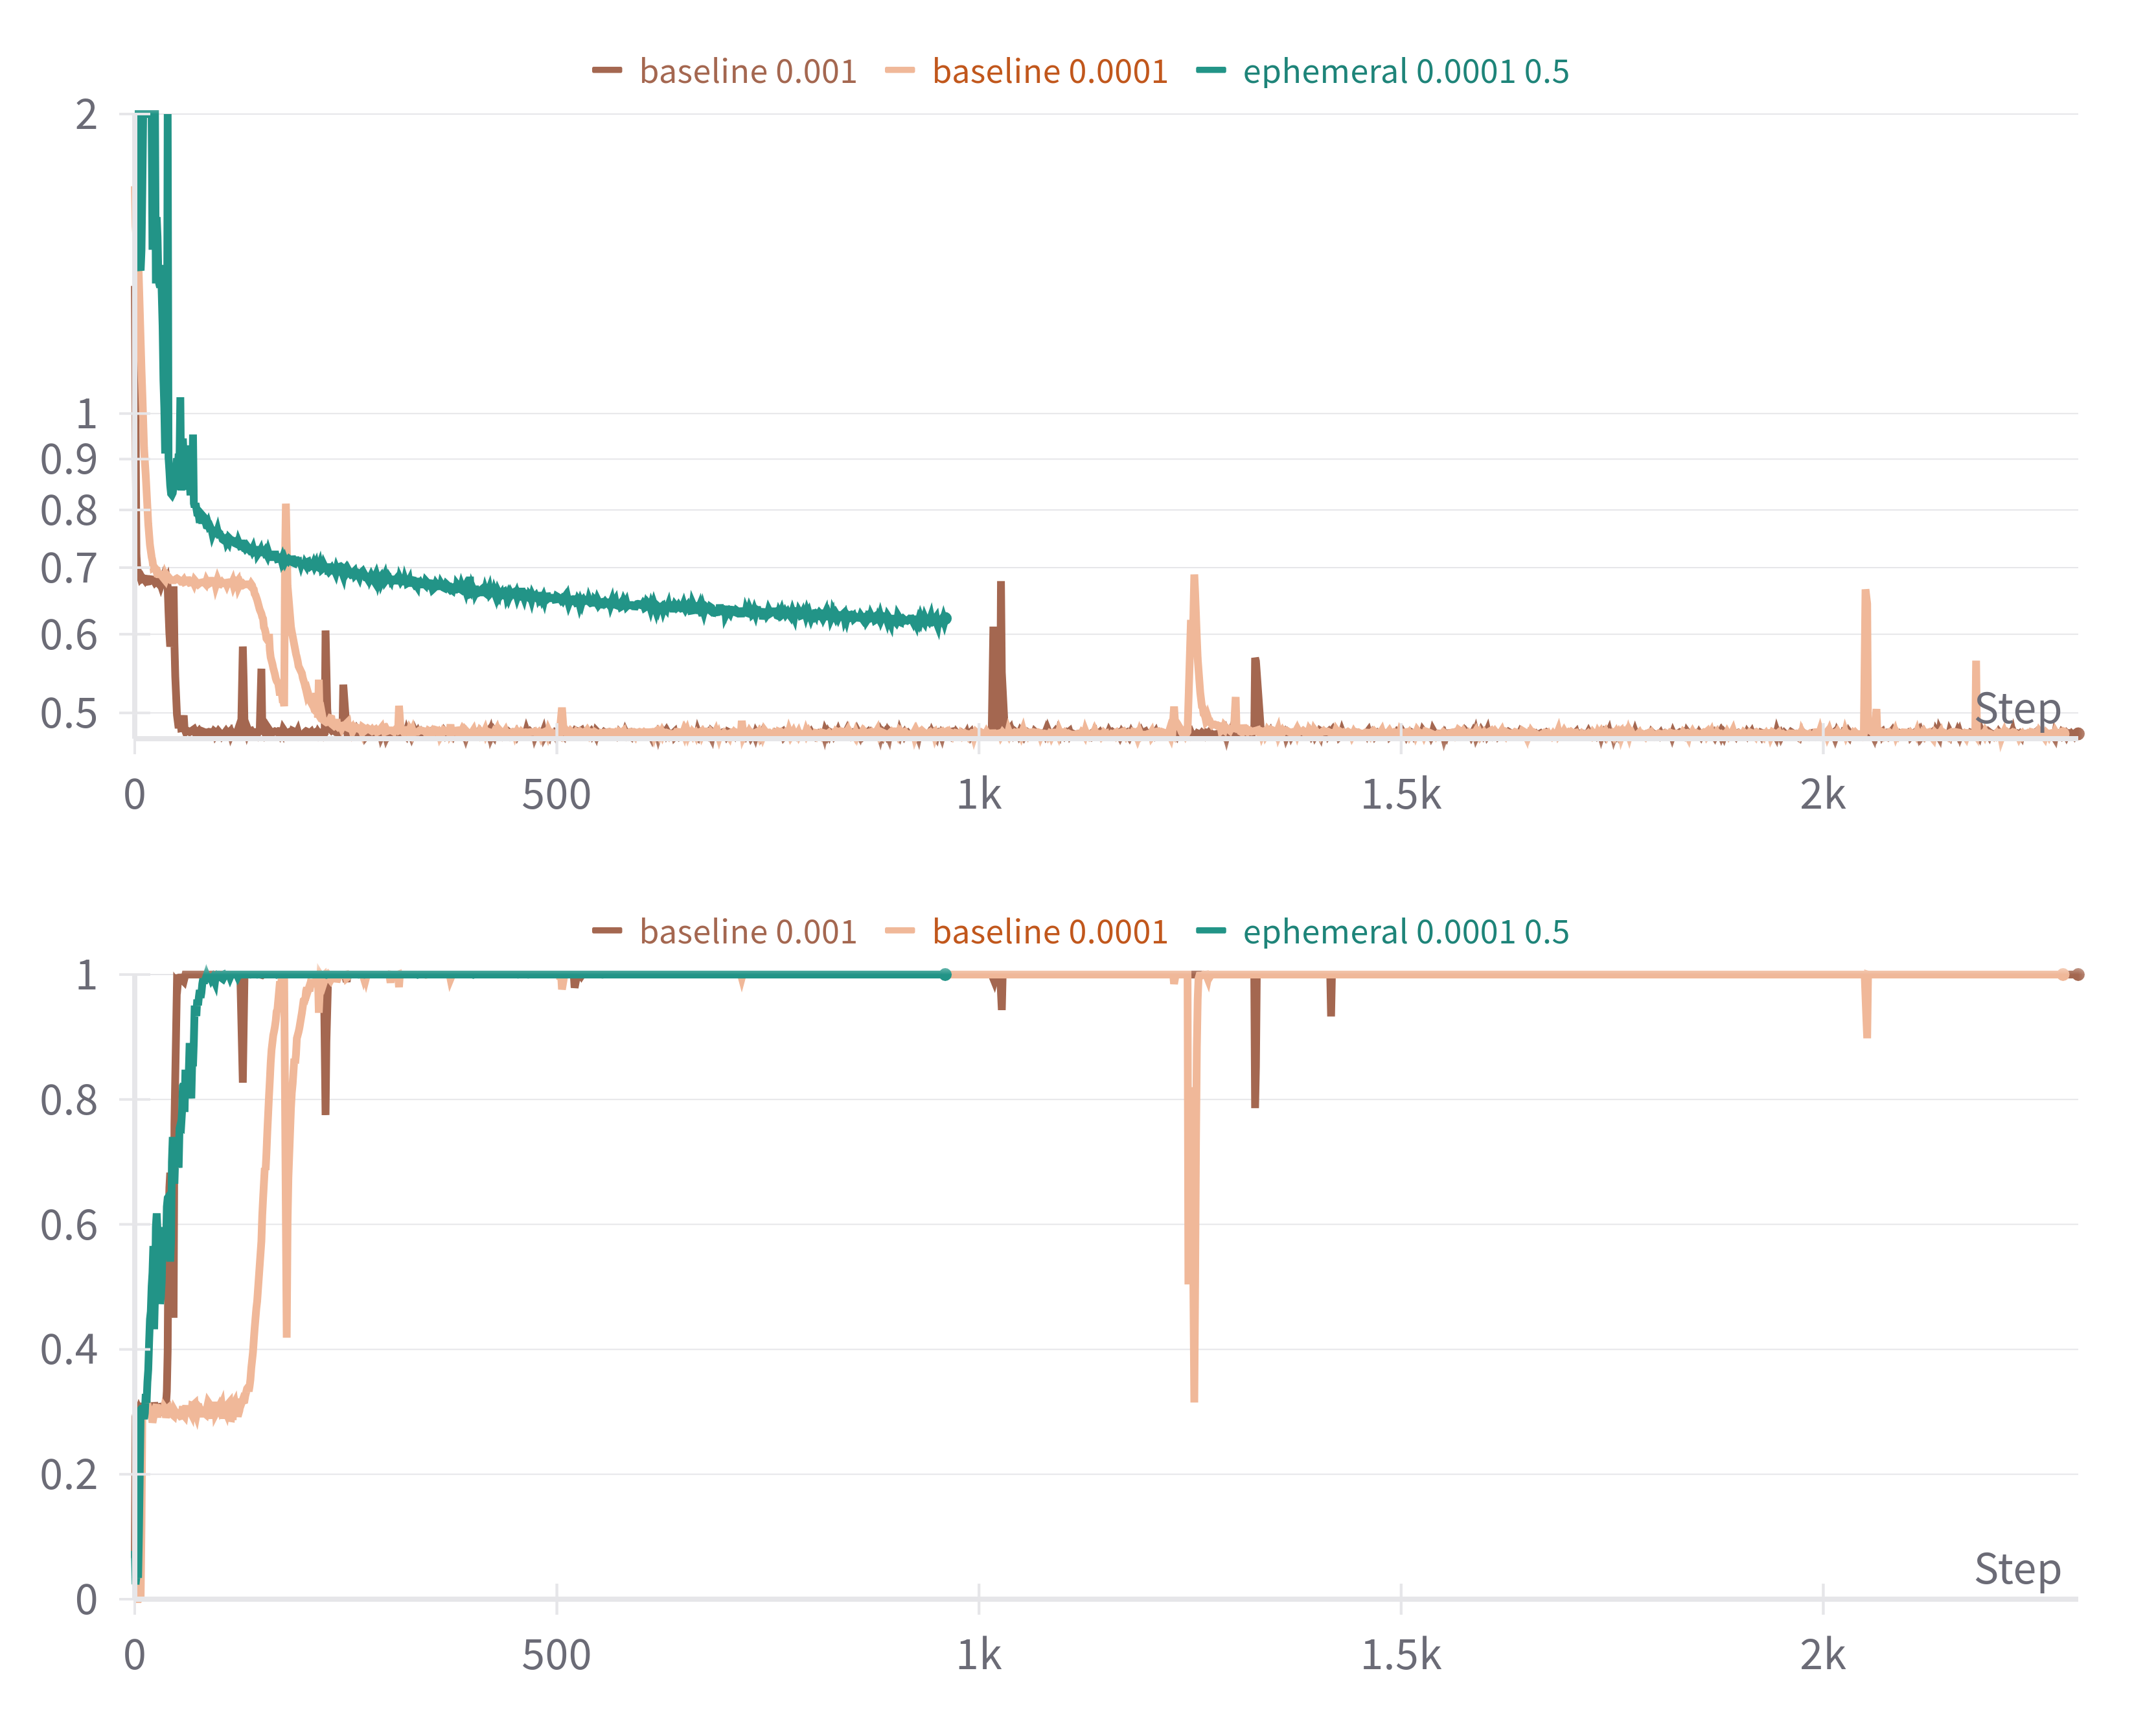
\includegraphics[width=0.8\linewidth]{figure_1.png}
\caption{Baseline runs display the learning rate beside them, and ephemeral runs include the forget rate, as well. The first graph shows the loss, and the bottom graph displays the model's prediction accuracy. The baseline RNN achieves a lower loss value, and remains stable enough for a higher learning rate to be used, but Ephemeral Weights converges to a high accuracy before the baseline does, when the same learning rate is used and its forget rate is tuned well. Under experimental implementations, Ephemeral Weights does not compute as many steps in the same amount of time, but remains remarkably stable.}
\label{fig:key_recall}
\end{center}
\end{figure}

\subsection{Repeated Sequences}
A synthetic dataset of one to four randomly chosen characters repeated until the character limit. The ability to train this task indicates that the memory storage mechanism is capable of storing several input-output associations. 

\begin{figure}[h]
\begin{center}
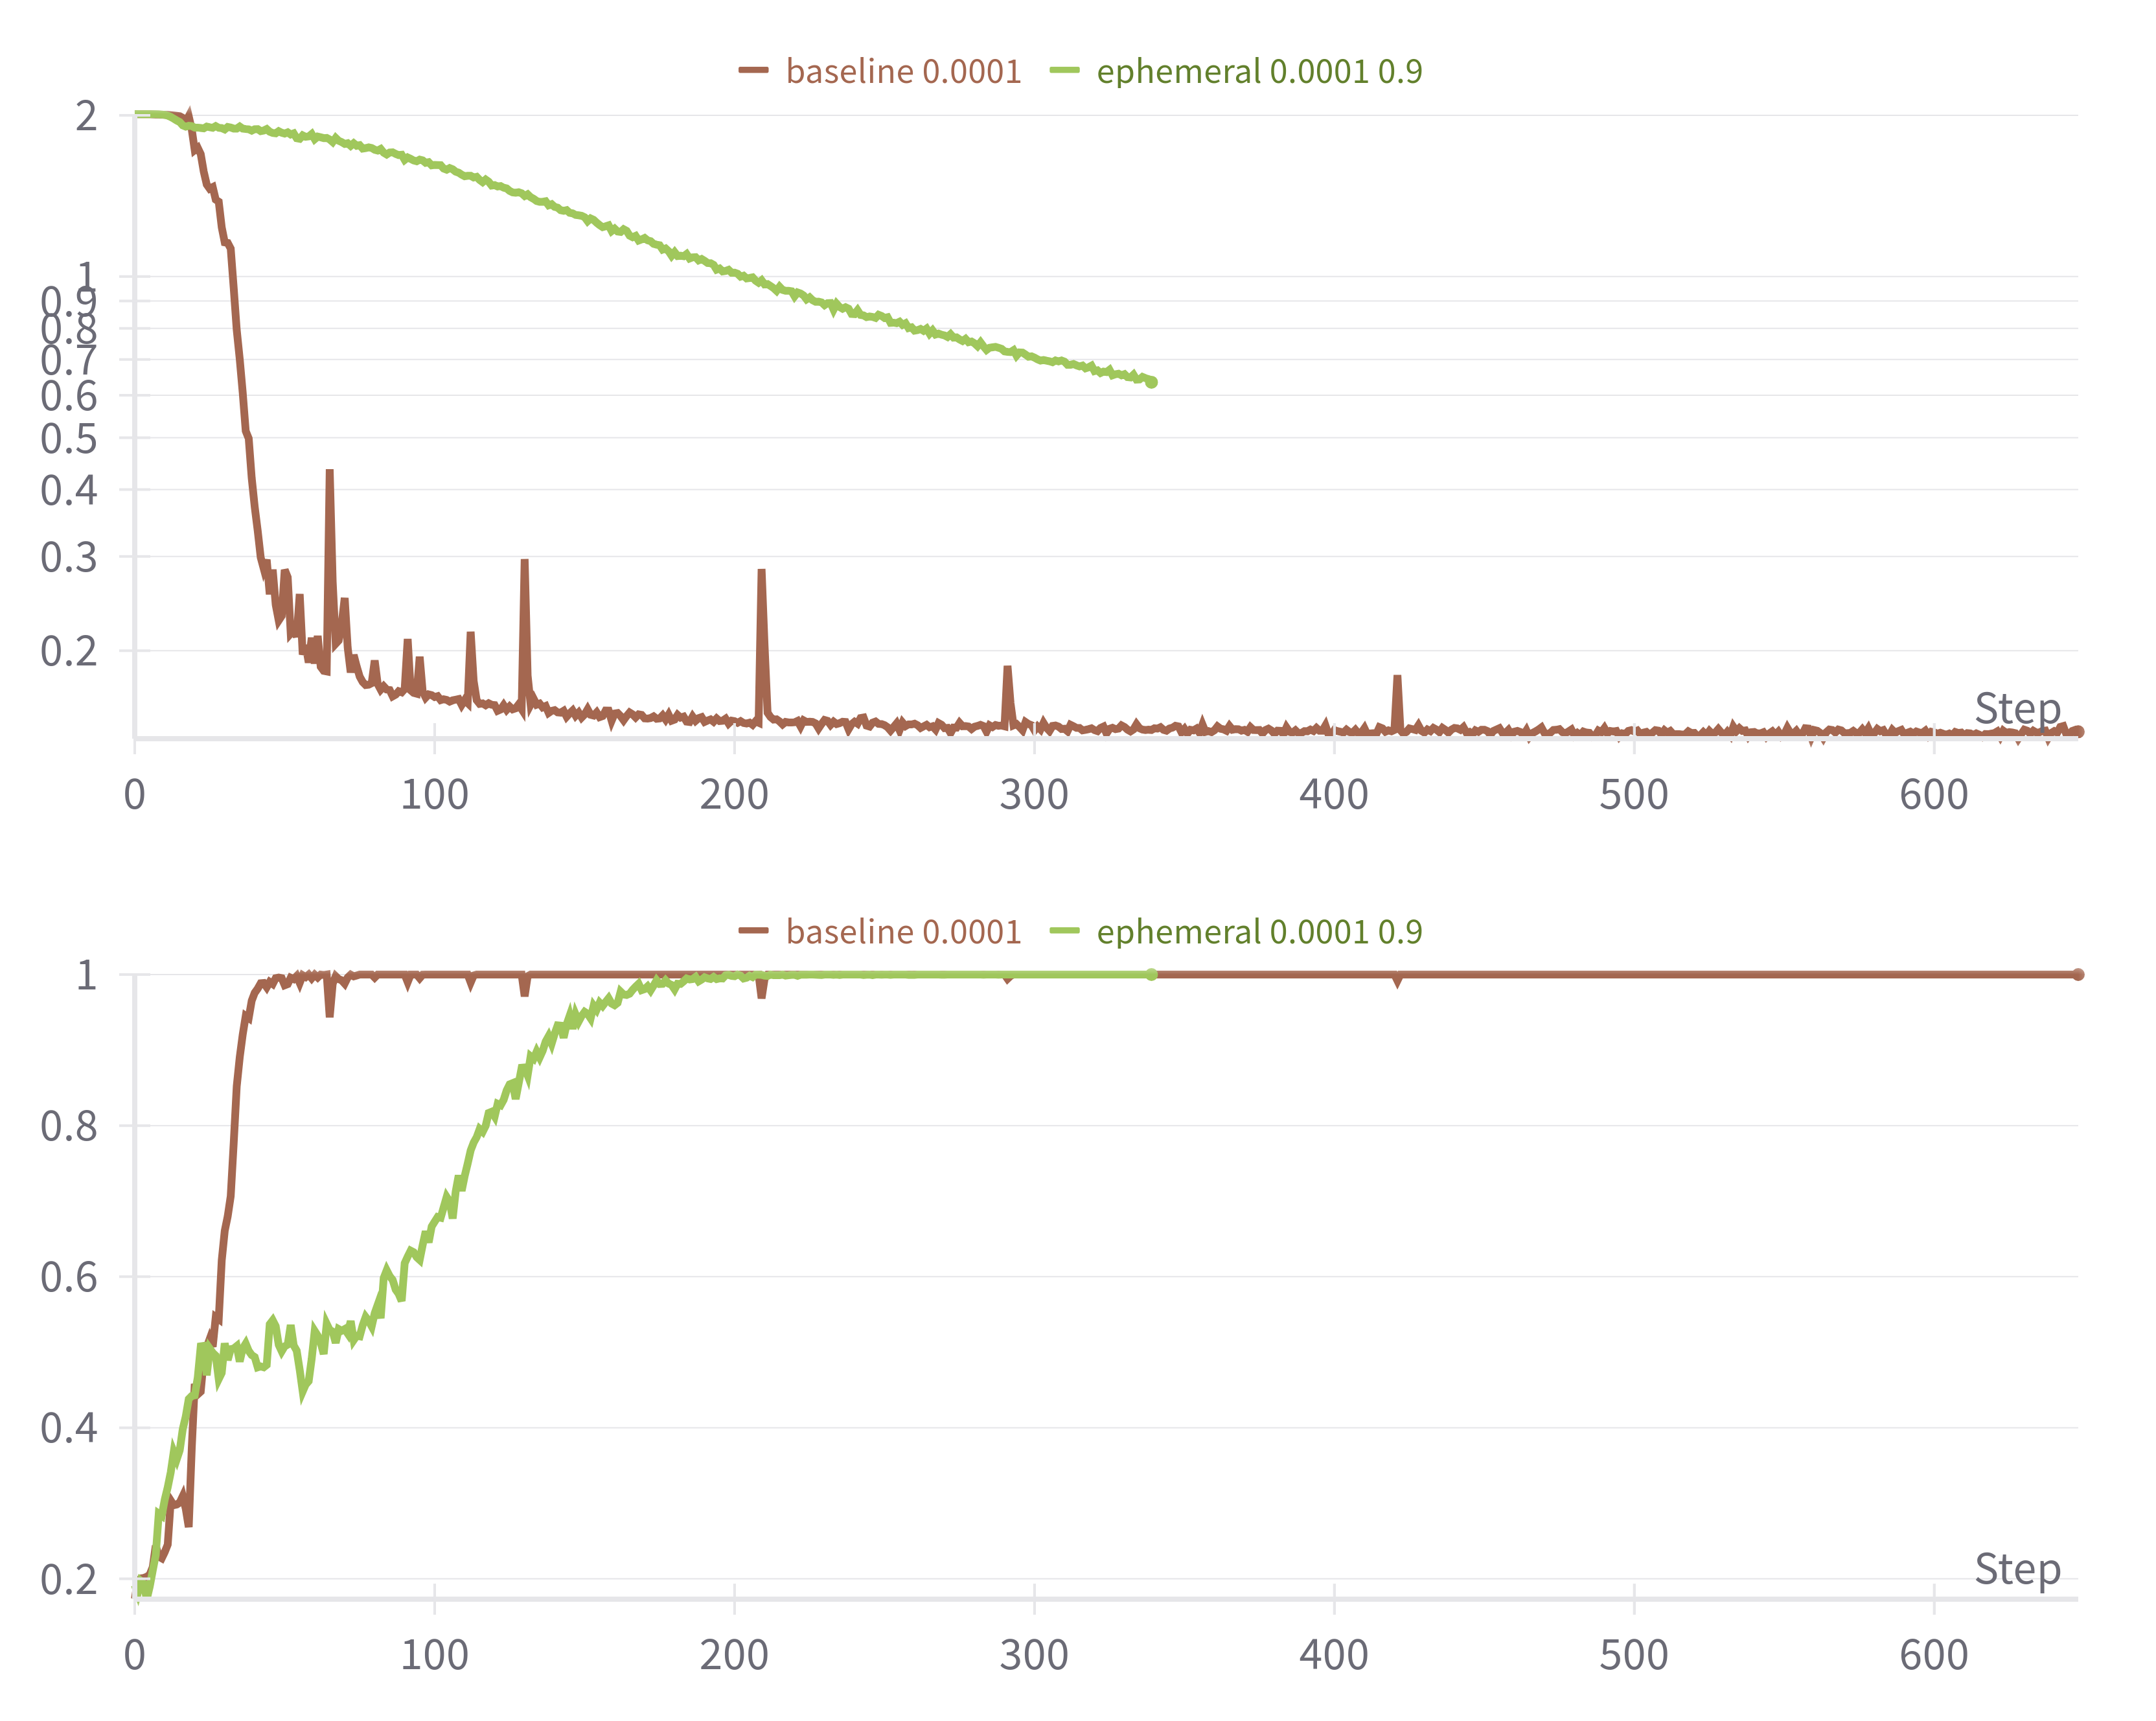
\includegraphics[width=0.8\linewidth]{figure_2.png}
\caption{The baseline, traditional RNN with backprop is used as a benchmark, converging quickly on the loss values and accuracy. Ephemeral weights converge more slowly, but do so without any recurrent connection.}
\label{fig:repeated_sequences}
\end{center}
\end{figure}

\subsection{Palindromes}
A synthetic dataset of random-character palindromes tests the model's ability to perform more complex memory operations. In this next-character prediction task, the model must recall the first half of characters in reverse order to complete the palindrome. Some examples:
\begin{verbatim}
abcba
xyzyx
12321
qwerttrewq
\end{verbatim}

This task goes beyond simple associative retrieval, requiring the network to not only store character associations but also retrieve them in inverted order. The reversal operation demands both memory storage and transformation capabilities, making it significantly more challenging than key-recall or repeated sequences.

\begin{figure}[h]
\begin{center}
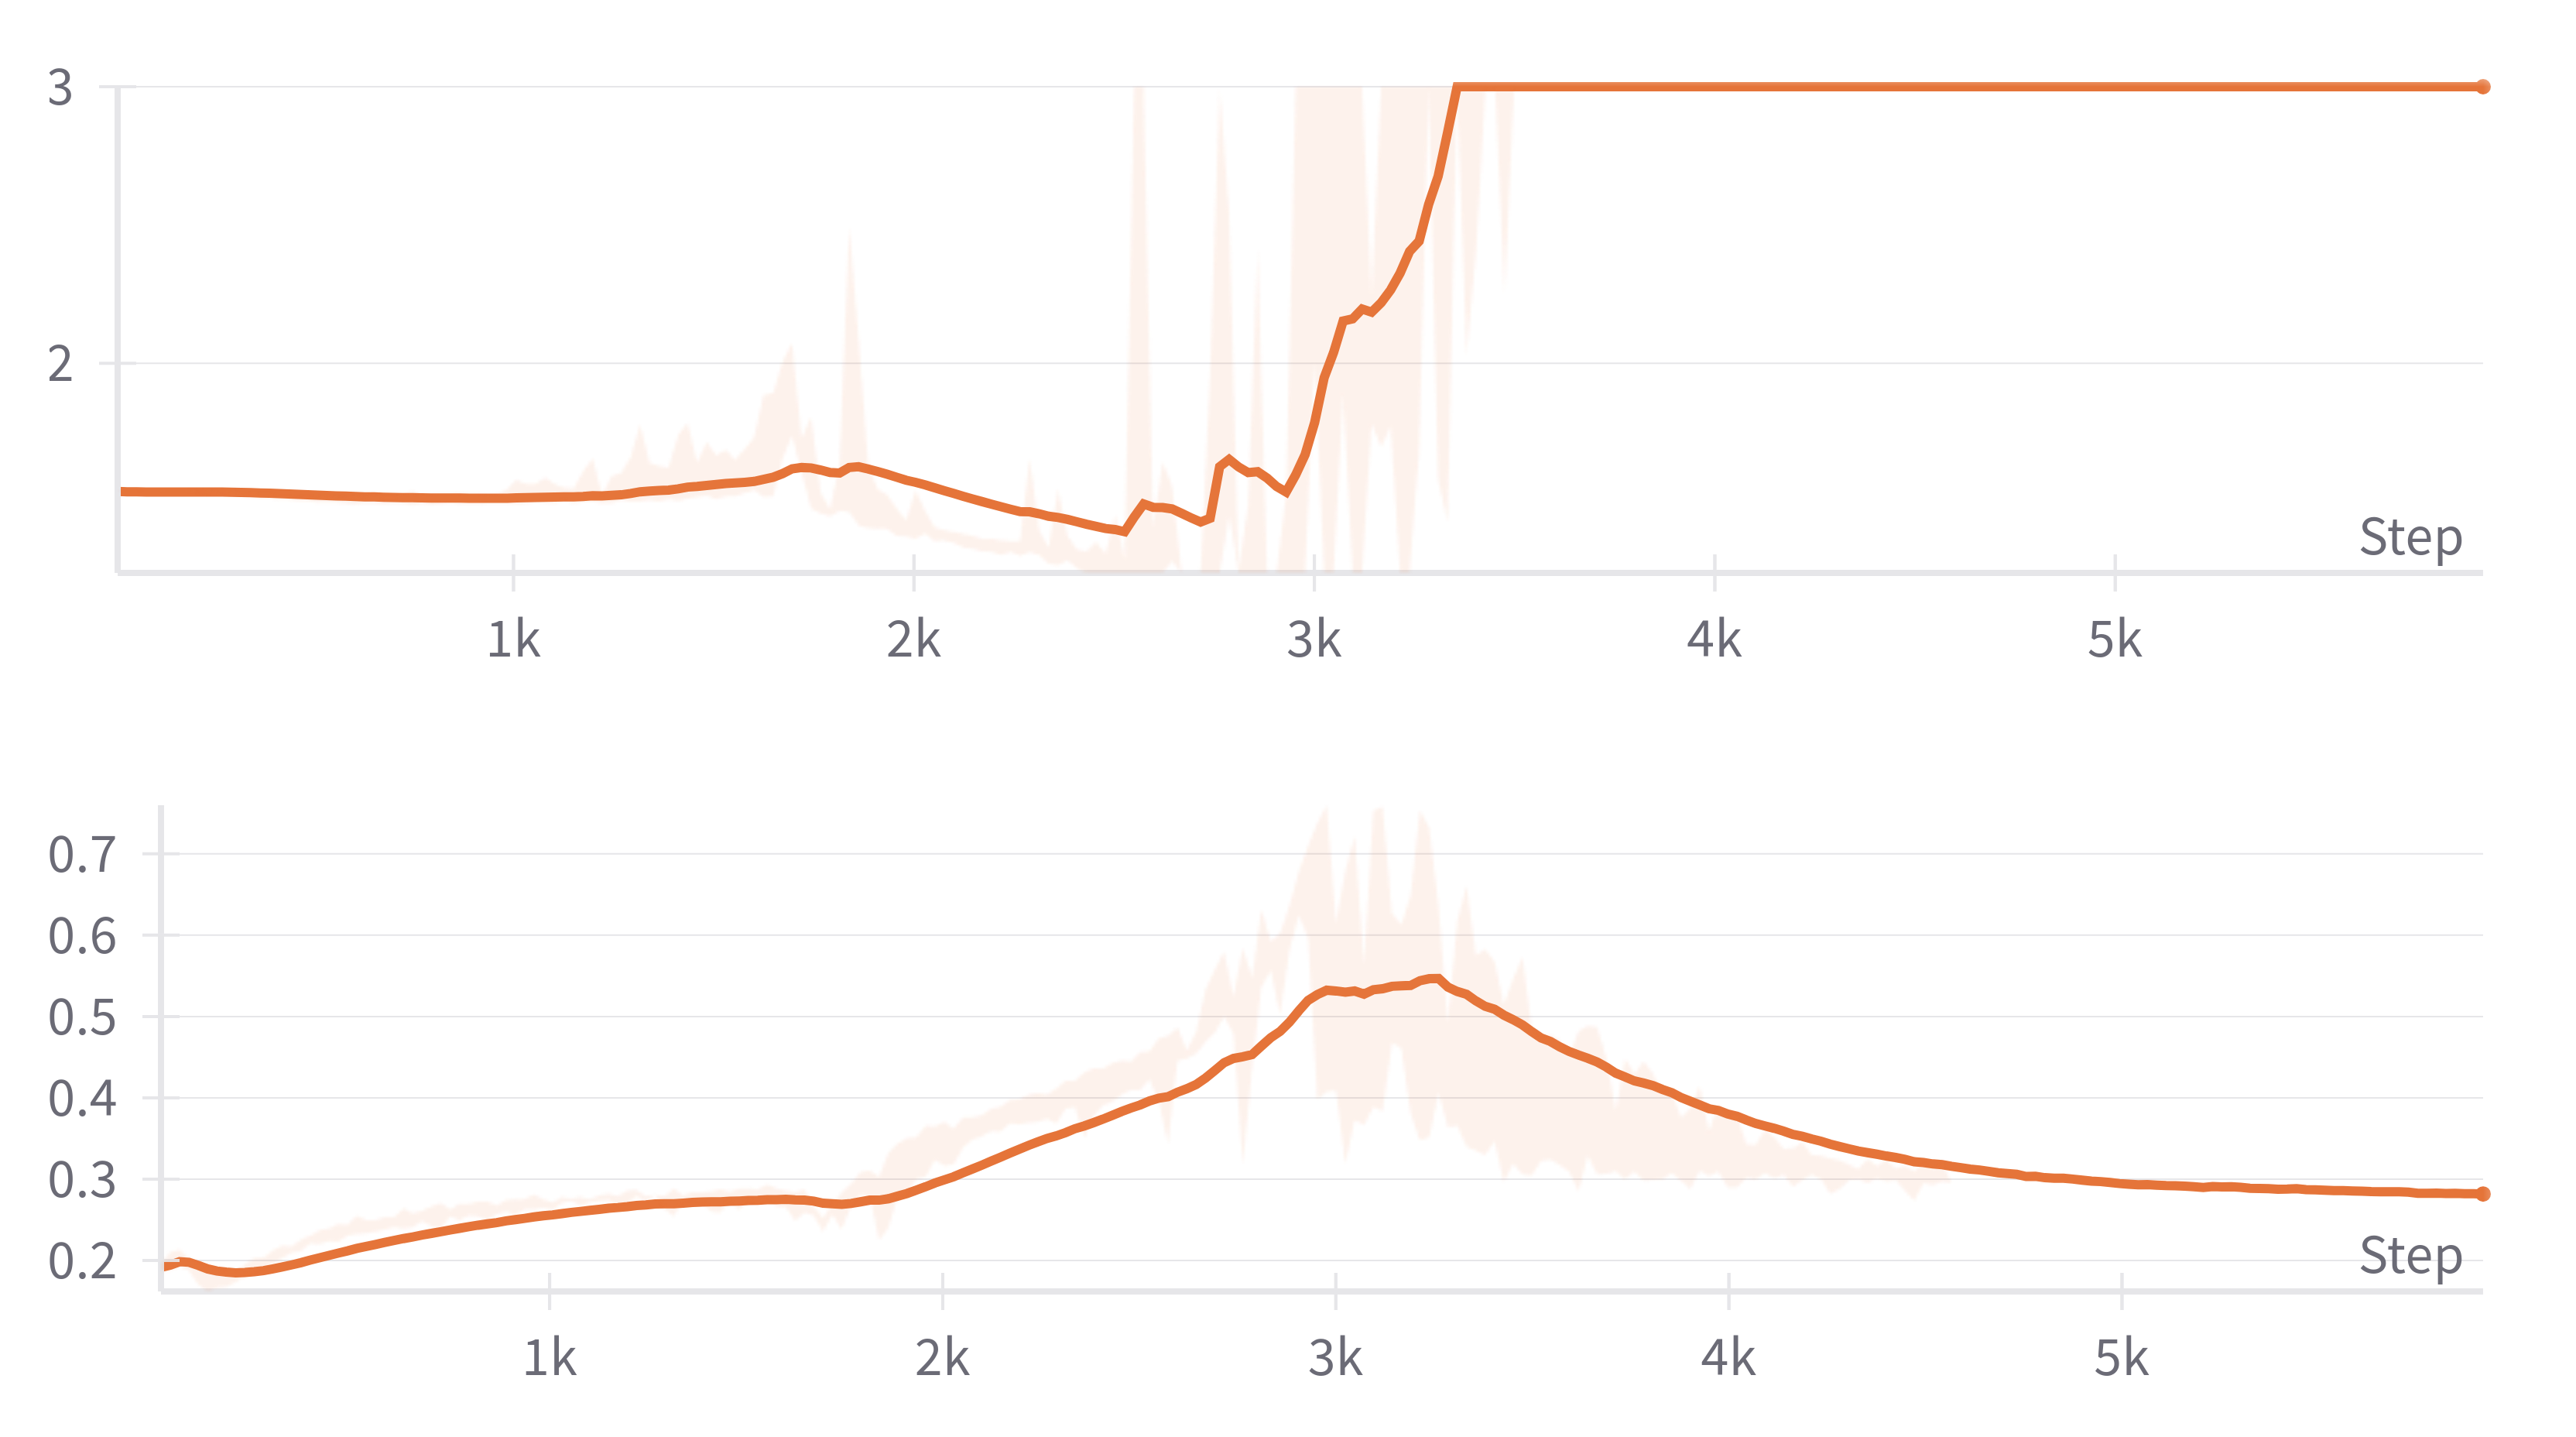
\includegraphics[width=0.8\linewidth]{figure_3.png}
\caption{Ephemeral weights demonstrate characteristic volatility on the palindromes task, reaching accuracy as high as 0.75 before experiencing gradient explosion and failure. This pattern illustrates the inherent instability that can emerge with synthetic datasets that create particularly steep loss landscapes.}
\label{fig:palindromes}
\end{center}
\end{figure}

\subsubsection{Volatility Emergence and Gradient Explosion}

The palindromes task reveals a fundamental challenge with ethereal weights: their susceptibility to gradient explosion under certain conditions. As shown in Figure 3, the model can achieve promising accuracy (up to 0.75) before experiencing catastrophic failure characterized by rapidly increasing loss and plummeting accuracy. This volatility pattern is particularly pronounced with synthetic datasets, which tend to create non-smooth, "bumpy" loss landscapes that amplify the destabilizing effects of rapid weight changes.

Our analysis reveals that gradient explosion in ethereal weights follows a predictable pattern driven by the ratio of gradient norms between high-plasticity and low-plasticity weights. In stable training runs, this gradient ratio tends to shrink over time as the slower weights provide stabilizing influence. However, in models that eventually explode, the gradient ratio consistently grows from the start, indicating that high-plasticity weights are gaining disproportionate influence over the network's behavior.

This observation suggests that gradient explosion in ethereal weights is not merely a case of traditional exploding gradients, but rather a feedback loop where high-plasticity weights exploit the learning objective in an uncontrolled manner. The rapid weight changes create increasingly large gradient signals, which in turn drive even more extreme weight updates, creating a runaway process that overwhelms the stabilizing influence of slower weights.

\subsubsection{Hyperparameter Dependencies and Effective Learning Rate}

The stability of the system depends on a delicate balance between multiple factors:

\textbf{Base Learning Rate}: Controls the only weights whose values truly persist across time steps. If these slow weights are too weak to provide adequate stabilizing influence over the more volatile high-plasticity weights, the system becomes unstable.

\textbf{High-Plasticity Learning Rate}: Creates a narrow operational window—too low and the model lacks effective working memory, too high and gradient explosion becomes inevitable.

\textbf{Ratio of High to Low-Plasticity Weights}: Typically set to 0.1 or 0.2, this ratio must provide sufficient capacity for associative memory storage while avoiding the instability that comes with too many volatile parameters.

\textbf{Forgetting Rate}: Must balance memory persistence with stability—too aggressive and ethereal memory disappears before it can be utilized, too conservative and gradient explosion becomes unavoidable.

A critical challenge is that appropriate values for these hyperparameters appear highly task-dependent, influenced by factors such as the required memory persistence duration, the density of information that must be stored in working memory, and the natural volatility of the dataset itself. This dependency on intensive hyperparameter tuning represents a significant limitation for practical applications.

A Hyperparameter sweep on the 3-character reversed sequence task indicated that the linear interaction of the base learning rate and the high-plasticity learning rate determnie the stability outcomes. It also indicated, in the same sweep, that of the two hyperparameters, high-plasticity learning rate is far more dominant in determining the accuracy of the model in the time-constrained training regime. Therefore, a balance must be struck, when choosing hyperparameters, setting the high-plasticity as high enough to enable effective memory encoding, but low enough to avoid instability (Figure 4).

\begin{figure}[h]
\begin{center}
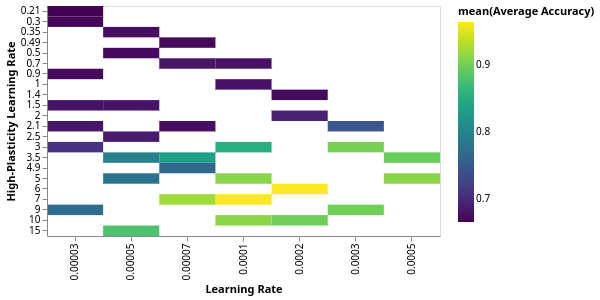
\includegraphics[width=0.8\linewidth]{figure_5.png}
\caption{Hyperparameter sweep results on the 3-character reversed sequence task showing the interaction between base learning rate and high-plasticity learning rate. The visualization demonstrates the linear relationship between these hyperparameters in determining stability outcomes, with the high-plasticity learning rate showing dominant influence over model accuracy in time-constrained training regimes.}
\label{fig:hyperparameter_sweep}
\end{center}
\end{figure}


\subsection{Volatility and Stability Analysis}

The ethereal weights mechanism exhibits characteristic volatility patterns that closely resemble exploding gradient phenomena. In both classical exploding gradients and our ethereal-weights volatility, instability stems from positive feedback in the update rule: as parameter magnitudes increase, the induced gradients scale up, amplifying subsequent updates unless explicit damping (e.g., weight decay, normalization, or clipping) keeps the effective gain below unity. Understanding these dynamics is crucial for practical implementation and reveals fundamental constraints of the approach.

\subsubsection{Gradient Explosion Dynamics}

The volatility manifests as a cascading failure where gradient norms and weight magnitudes accelerate simultaneously, leading to rapid increases in loss and corresponding drops in accuracy, as seen in Figure 3. This behavior appears intrinsic to the mechanism rather than a mere implementation artifact—the aggressive gradient amplification required for effective memory encoding creates inherent instability.

A key early warning indicator emerges from monitoring the ratio of gradient norms between high-plasticity and low-plasticity weights. Stability correlates with this ratio shrinking over time, while plateauing or growth of the ratio precedes explosive behavior. This observation aligns with the intuitive understanding that high-plasticity weights, when left unchecked by slower stabilizing weights, can enter a positive feedback loop where rapid changes amplify subsequent gradient signals.
(put a figure here showing gradient ratio over time for stable vs unstable runs)

Holding other hyperparameters constant, varying the base learning rate and the plasticity modifier reveals a linear boundary between stable and unstable regimes. Lower base learning rates allow for higher plasticity modifiers before instability arises, while higher base learning rates necessitate more conservative plasticity settings (Figure 6). A limitation of this experiment is that some runs that initially appear stable within the training timeframe still exhibit climbing loss numbers at the tail end, suggesting eventual instability if training were extended further. 
\begin{figure}[h]
\begin{center}
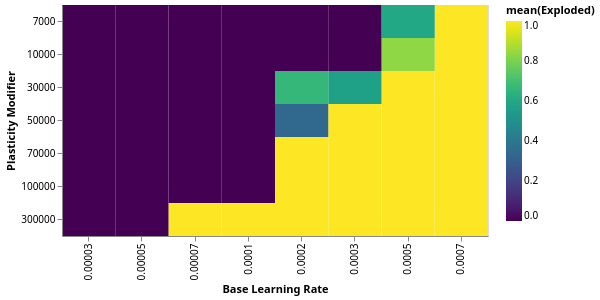
\includegraphics[width=0.8\linewidth]{figure_6.png}
\caption{Hyperparameter sweep results on the 3-character reversed sequence task showing the interaction between base learning rate and high-plasticity learning rate, 10 samples for each combination, on stability. A linear boundary separates runs that remained under a loss of 2 from those that underwent a runaway explosion of gradient values during a set number of training steps.}
\label{fig:hyperparameter_sweep_6}
\end{center}
\end{figure}

\subsubsection{Forgetting Rate Dynamics}

The forgetting rate mechanism proves essential but insufficient for complete stabilization. While aggressive forgetting rates prevent explosion, they also reduce memory duration below useful thresholds. Conversely, insufficient forgetting leads to inevitable instability. This creates a narrow operational window that varies significantly across tasks and datasets.

Synthetic datasets consistently exhibit more volatile behavior than natural text tasks, likely due to their non-smooth loss landscapes. The discrete, artificial nature of synthetic sequence tasks creates sharp loss cliffs that amplify the destabilizing effects of rapid weight changes, whereas natural language provides more gradual loss surfaces that better accommodate the ethereal weights mechanism.

\subsubsection{Stabilization Strategies}

Given the inherent volatility of ethereal weights, developing effective stabilization strategies becomes crucial for practical implementation. Our experiments reveal several approaches that can help balance stability with working memory effectiveness, though each comes with specific trade-offs.

\textbf{Gradient Propagation Method Selection}: Direct Feedback Alignment (DFA) emerges as the most effective approach for maintaining stability. Unlike standard backpropagation, which creates volatile feedback loops when plastic weights are used for both forward computation and gradient propagation, DFA employs fixed random feedback weights that remain constant throughout training. This architectural choice significantly reduces the positive feedback effects that lead to gradient explosion.

\textbf{Weight Clipping}: Constraining weight magnitudes through clipping proves highly effective when combined with standard backpropagation. By preventing weights from reaching extreme values, clipping helps contain the cascading effects that characterize gradient explosion. However, the same large weight magnitudes that threaten stability are often necessary for effective memory encoding. Overly aggressive clipping can therefore eliminate the model's working memory capabilities entirely, and turns out to be less useful when using DFA on more conservative choices of learning rate and ratio hyperparameters.
A hyperparameter sweep on the clipping threshold was performed on the 3-character reversed sequence task, on selections of base learning rate and high-plasticity learning rate that were known to be on the edge of stability without clipping. The results were inconclusive, with 10 samples each on values between 0.01 and 100 showing no clear pattern of better stability or accuracy. This suggests that while weight clipping can help prevent explosion, its optimal setting is highly data-dependent.

\textbf{Periodic Memory Reset}: Wiping high-plasticity weights after sequence completion provides a hard reset mechanism that prevents the accumulation of destabilizing weight values across sequences. This approach proves particularly effective for tasks with clear sequence boundaries, essentially treating each sequence as an independent working memory episode. While this prevents cross-sequence contamination, it also eliminates any potential benefits from longer-term memory consolidation.

\textbf{Ineffective Approaches}: Several commonly used stabilization techniques prove counterproductive with ethereal weights. Gradient clipping, despite its effectiveness in traditional neural networks, fails because the memory mechanism fundamentally depends on occasional large gradient magnitudes to encode information effectively. Similarly, batch normalization and layer normalization actively harm performance by normalizing away the bimodal gradient distribution that enables memory encoding—the extreme gradient magnitudes these techniques suppress are precisely what makes ethereal weights functional.

\textbf{Dataset Choice}: The choice of training data significantly impacts stability requirements. Natural language tasks, with their relatively smooth loss landscapes, suffer less readily from the volatile dynamics observed in this paper. 

\textbf{Extended Training Regimes}: Some models exhibit U-shaped learning curves where initial gradient explosion eventually stabilizes after sufficient training. This phenomenon suggests that the optimization landscape contains stable regions accessible only after traversing unstable phases. While intriguing, this approach remains impractical for most applications due to the computational cost and unpredictability of the stabilization process.

\textbf{Hyperparameter Co-optimization}: The most promising long-term approach involves developing principled methods for jointly optimizing the base learning rate, plasticity modifiers, forgetting rates, and plasticity ratios. Current approaches rely heavily on task-specific hyperparameter sweeps, but future work should explore meta-learning approaches or adaptive mechanisms that can automatically balance stability and memory effectiveness across different tasks and datasets.

The fundamental challenge remains that ethereal weights operate in a narrow stability regime where effective memory encoding and system stability are in constant tension. Future implementations will likely require sophisticated control mechanisms that can dynamically adjust these parameters based on real-time monitoring of gradient ratios and other stability indicators.

\subsubsection{Effective Learning Rate Paradox}

An intriguing phenomenon emerges when calculating the effective learning rate across all parameters. Despite theoretical expectations, effective learning rates that would cause immediate explosion in traditional RNNs (often exceeding 20 in synthetic tasks) prove workable with ethereal weights. This paradox suggests that the forgetting mechanism fundamentally alters the learning dynamics, creating a different stability regime than conventional gradient descent.

However, this effective learning rate metric fails to correlate strongly with actual performance or stability, indicating that the temporal dynamics of forgetting introduce complexities not captured by simple averaging approaches. The ethereal component of the learning process appears to operate under different mathematical principles than standard parameter optimization.

\subsection{Preservation of Long-Term Learning}

A critical concern with the ethereal weights approach is whether the volatile behavior of high-plasticity weights interferes with the stable, long-term learning that should occur in the low-plasticity parameters. Our analysis demonstrates that these two learning processes can coexist effectively, with each operating at its designated timescale without mutual interference.

\begin{figure}[h]
\begin{center}
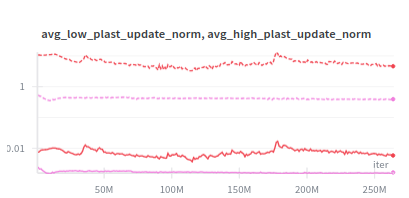
\includegraphics[width=0.8\linewidth]{figure_4.png}
\caption{Gradient norm evolution throughout training shows clear separation between high-plasticity and low-plasticity weight categories. The high-plasticity weights (red) exhibit characteristic volatility with occasional spikes corresponding to memory encoding events, while low-plasticity weights (blue) maintain steady, controlled gradient magnitudes. This separation demonstrates that the two learning processes operate independently, allowing stable long-term learning to proceed alongside volatile working memory encoding.}
\label{fig:gradient_norms}
\end{center}
\end{figure}

Figure 5 reveals that gradient norms for high-plasticity and low-plasticity weights remain highly distinct throughout training, indicating that the two categories of parameters operate in separate dynamic regimes. The high-plasticity weights exhibit the expected volatility with occasional large spikes corresponding to memory encoding events, while the low-plasticity weights maintain steady, controlled gradient magnitudes characteristic of stable optimization.

This separation is crucial for the dual-timescale learning hypothesis underlying ethereal weights. The steady decrease in loss observed across our experiments suggests that the model continues to learn long-term patterns at the low-plasticity learning rate while simultaneously managing working memory at the high-plasticity rate. This dual-process behavior indicates that ethereal weights successfully implement a form of multi-timescale learning where different parameter subsets serve distinct functional roles.

The preservation of long-term learning can be attributed to several factors. First, the random assignment of plasticity levels ensures that the network's fundamental computational capacity remains largely intact, with only a small fraction (typically 10-20\%) of parameters dedicated to volatile memory functions. Second, the forgetting mechanism prevents high-plasticity weights from accumulating permanent biases that could interfere with the network's overall optimization trajectory.

To rigorously test this dual-learning hypothesis, future experiments could implement a controlled study where models are trained on a primary task (e.g., language modeling) while periodically exposed to working memory challenges (e.g., key-recall sequences). By measuring performance on both the primary task and working memory tasks throughout training, researchers could quantify how effectively the two learning processes coexist. Additionally, ablation studies could examine performance when high-plasticity weights are periodically frozen or reset, allowing direct measurement of the low-plasticity weights' learning progress in isolation.

Another promising experimental approach would involve training ethereal weights models on tasks with known long-term dependencies (such as copying tasks with very long delays) while simultaneously requiring short-term memory operations. Success on both components would provide strong evidence that the architecture can maintain stable long-term learning while providing functional working memory capabilities.

The implications of this dual-timescale learning extend beyond the immediate applications of ethereal weights. This approach suggests a general framework for neural architectures that can simultaneously optimize for different temporal objectives, potentially offering new approaches to continual learning, meta-learning, and adaptive systems that must balance stability with flexibility.

\section{Discussion}

\subsection{Ethereal Weights as Functional Working Memory}

Our experiments demonstrate that ethereal weights successfully encode functional working memory without explicit gatekeeping mechanisms. Unlike traditional memory architectures that employ gates, attention mechanisms, or explicit memory curation, ethereal weights operate through pure associative storage of recent gradient updates. This approach can reliably hold multiple pieces of information simultaneously—our experiments confirm storage of at least three distinct items—with positional encoding providing additional organizational structure.

The memory mechanism operates as an associative system that performs best with strong retrieval cues, though the temporal decay ("age") of stored information can also serve as an effective retrieval mechanism. This dual-access pattern mirrors biological working memory, where both content-based and temporal-based retrieval strategies coexist. However, the associative nature of this memory system also reveals its limitations: while effective for storage and retrieval, it lacks inherent mechanisms for information transformation or manipulation, as evidenced by the challenges with palindrome tasks that require sequence reversal.

The volatility characteristics discussed in Section 4.4 are intrinsically linked to this memory function. The gradient explosion patterns that threaten stability are not merely implementation artifacts but fundamental consequences of the memory encoding mechanism. The aggressive gradient amplification required for rapid memory formation creates a delicate balance between effective encoding and system stability, suggesting that volatility management is an essential component of any practical ethereal weights implementation.

\subsection{Toward a Multi-Scale Memory Pipeline}

The current ethereal weights approach represents only one component of what could become a comprehensive memory hierarchy. The limitations observed in our experiments—particularly the lack of information selection and the challenges with complex transformations—suggest that ethereal weights are best understood as part of a larger memory pipeline rather than a complete solution.

We envision a biologically-inspired memory architecture that operates across multiple timescales: context windows for immediate information access, recurrent connections for short-term rehearsal loops, high-plasticity weights for rapid encoding, medium-plasticity weights for intermediate storage, and low-plasticity weights for long-term consolidation. This hierarchy mirrors human memory processes, where information flows from immediate perception through various stages of consolidation.

Consider the analogy of remembering a phone number: humans typically have an immediate context window of approximately four digits, requiring active rehearsal (analogous to recurrent loops) to maintain longer sequences. With repetition, the number can be retained for minutes (high-plasticity storage), and with further practice, it may persist for hours or days (medium-plasticity) before potentially becoming permanently encoded (low-plasticity). Each stage serves a specific function in the overall memory system.

This multi-scale approach could enable emergent memory consolidation behaviors similar to replay buffers in reinforcement learning or bootstrapped fine-tuning in language models. A conversational AI system might initially store user preferences in context windows, transfer frequently mentioned preferences to recurrent loops, gradually encode them in high-plasticity weights, and eventually consolidate important patterns into the model's long-term parameters. This would create a natural progression from ephemeral working memory to permanent knowledge, freeing up short-term memory resources for new information.

The key insight is that effective memory systems require not just storage mechanisms but also information selection and consolidation processes. Future work should explore how attention-like mechanisms or learned gating functions could be integrated with ethereal weights to create more sophisticated memory management systems.

\subsection{Bridging Manual Memory Storage and Parameter-Based Memory}

Parameter-based memory is stored over the course of the pretraining of the model, encoding patterns, grammar rules, and facts from large text datasets, for example. Memory stored manually is stored by the model or the software built around the model, either by maintaining context windows or by recurrent connections. It is quite distinct from parameter-based memory under the current paradigm. Ephemeral weights show that there may exist a more gradual transition from the more manually stored memory to parameter-based memory. 

Future work should focus on plasticity values that are more dynamically selected, perhaps via a metalearning outer loop. Variable, more sophisticated learning rates may be selectable based off of only information available pre-training, such as the magnitude of high-plasticity values. Biologically-inspired learning rules beyond standard backpropagation, such as Hebbian plasticity, may stabilize volatile learning caused by ephemeral weights. A more rigorous examination of the dynamics between the forgetting rate, the ratio of ephemeral to slow weights, the plasticity of the ephemeral weights, and the base learning rate, will allow for a more principled selection of their values instead of large hyperparameter sweeps.

The potential applications extend beyond basic memory storage to alignment and continual learning scenarios. A language model capable of continuous parameter-based adaptation could naturally adjust to individual user preferences and requirements, creating more personalized and responsive AI systems. The smooth transition from short-term to long-term memory storage could enable AI agents to maintain coherent long-term projects spanning days or weeks, rather than being limited to the immediate context of individual conversations.

\section{Conclusion}

This paper demonstrates that short-term memory in neural networks can be effectively stored in rapidly adapting parameters, without relying on traditional recurrent connections. By designating a small fraction of weights as "ephemeral"—with high plasticity and controlled forgetting rates—we enable the network to encode contextual information directly in its parameters through standard backpropagation. Our approach succeeds on key-recall and repeated sequence tasks, establishing that parameter-based working memory can function as an effective alternative to traditional recurrent architectures while revealing important insights about the dynamics and implementation requirements of such systems.

This work blurs the lines between traditional parameter-based memory (encoded during pretraining) and manually stored memory (maintained through recurrent connections or attention mechanisms). Ephemeral weights represent a middle ground based on biological plasticity, where information storage exists on a continuum of timescales rather than a binary distinction between training and inference.

Future work should explore dynamic plasticity parameters, variable forgetting rates, and hybrid architectures combining ephemeral weights with traditional memory mechanisms, such as Hebbian learning rules. Incorporating multiple timescales of parameter adaptation may lead to more efficient, adaptable systems that better mirror the flexibility of biological memory.

The potential for this work extends to alignment and continual learning applications. A language model that is capable of continuous alignment in a more biologically plausible way has the potential to adapt more closely to individuals' needs in an ever-refining way. Smooth transitions from short to long-term memory, stored efficiently in model parameters will grant AI a new modality for computing problems over varying timescales, opening up larger and more complex projects to AI assistance. The possibilities include agents capable of coherently planning and orchestrating projects over the course of days and weeks, rather than minutes.

\bibliography{collas2025_conference}
\bibliographystyle{collas2025_conference}

\end{document}
